\documentclass{ximera}
\usepackage{OERLinearAlgebra}


\usepackage{mathtools}

\author{Anna Davis \and Paul Zachlin} \title{Planes in $\RR^3$} \license{CC-BY 4.0}

\begin{document}

\begin{abstract}
  We establish that a plane is determined by a point and a normal vector, and use this information to derive a general equation for planes in $\RR^3$.
\end{abstract}
\maketitle

\section*{Equations of Planes}
{\color{red} Adapted from Nicholson Section 4.2}

You are probably familiar with the expression ``two points determine a line."  A line is also determined by one point and a vector parallel to the line.  You are probably also familiar with the fact that three non-collinear points determine a plane (This is why photographers use tripods for stability, while four-legged chairs often wobble!)  Is there another way to determine a plane?  

It is evident geometrically that among all planes that are perpendicular 
to a given straight line there is exactly one containing any given 
point. The diagram below shows several planes perpendicular to vector $\vec{u}$.  There are infinitely many such planes, but only one contains point $P$.

 \begin{image}[2.5in]
\tdplotsetmaincoords{70}{130}
	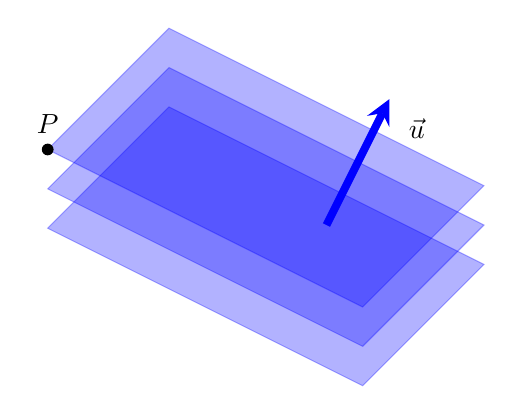
\begin{tikzpicture}[scale=1]

\filldraw[blue, opacity=0.3] (2,-1,2)--(2,-1,-2)--(-2,1,-2)--(-2,1,2)--cycle;

\filldraw[blue, opacity=0.3] (2,-0.5,2)--(2,-0.5,-2)--(-2,1.5,-2)--(-2,1.5,2)--cycle;

\filldraw[blue, opacity=0.3] (2,-1.5,2)--(2,-1.5,-2)--(-2,0.5,-2)--(-2,0.5,2)--cycle;

    \draw[->,line width=1mm, -stealth, blue](0,-1,-2)--(0.8,0.6,-2) ;%normal to grey
    \node[fill,circle,inner sep=1.5pt,label={$P$}] at (-2,1.5,2) {};
    \node[label={below right:$\vec{u}$}] at (0.8,0.6,-2) {};
     \end{tikzpicture}
          
     \end{image}

\begin{definition}[Normal Vector]\label{def:normalvectoplane}
A nonzero vector $\vec{n}$ is called a \dfn{normal} for a plane if it is orthogonal to every vector in the plane.
\end{definition}

\begin{example}
The standard unit vector $\vec{k}$ is orthogonal to every vector in the $xy$-plane, therefore it is a normal for the $xy$-plane.

\begin{image}[2in]
\tdplotsetmaincoords{70}{130}
	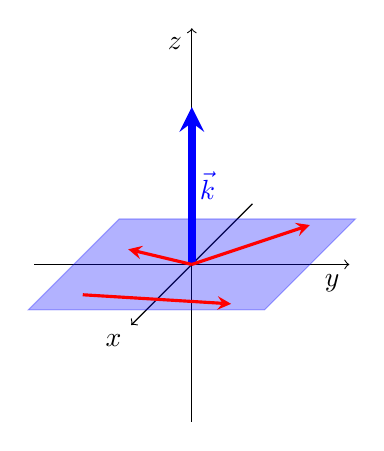
\begin{tikzpicture}[scale=1]

\draw[->](-2,0,0)--(2,0,0) node[below left]{$y$};
    \draw[->](0,-2,0)--(0,3,0) node[below left]{$z$};
    \draw[->](0,0,-2)--(0,0,2) node[below left]{$x$};
\filldraw[blue, opacity=0.3] (1.5,0,1.5)--(-1.5,0,1.5)--(-1.5,0,-1.5)--(1.5,0,-1.5)--cycle;
   	
    \draw[->,blue,line width=1mm, -stealth](0,0,0)--(0,2,0) ;
    
    \node[blue] at (0.2, 1, 0)   {$\vec{k}$};

\draw[->,line width=0.4mm, -stealth, red](0,0,0)--(1,0,-1.3) ;

\draw[->,line width=0.4mm, -stealth, red](-1,0,1)--(1,0,1.3) ;

\draw[->,line width=0.4mm, -stealth, red](0,0,0)--(-1,0,-0.5) ;

\end{tikzpicture}
\end{image}
\end{example}

Given a point $P_{0} = P_{0}(x_{0}, y_{0}, z_{0})$ and a nonzero vector $\vec{n}$, there is a unique plane through $P_{0}$ with normal $\vec{n}$.

\begin{image}[3.5in]
\tdplotsetmaincoords{70}{130}
	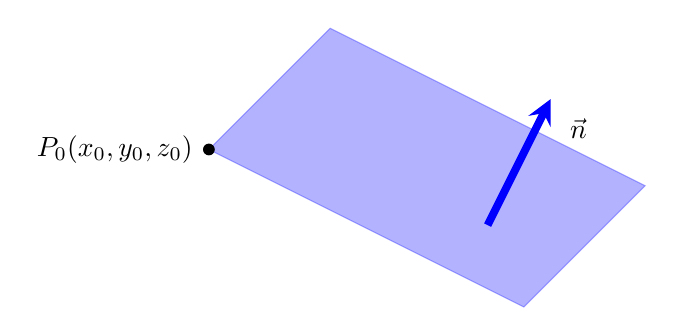
\begin{tikzpicture}[scale=1]

\filldraw[blue, opacity=0.3] (2,-0.5,2)--(2,-0.5,-2)--(-2,1.5,-2)--(-2,1.5,2)--cycle;

    \draw[->,line width=1mm, -stealth, blue](0,-1,-2)--(0.8,0.6,-2) ;%normal to grey
    \node[fill,circle,inner sep=1.5pt,label={left:$P_0(x_0, y_0, z_0)$}] at (-2,1.5,2) {};
    \node[label={below right:$\vec{n}$}] at (0.8,0.6,-2) {};
     \end{tikzpicture}
          
     \end{image}

This fact can be used to give a very simple description of a 
plane.
 Observe that a point $P = P(x, y, z)$ lies on this plane if and only if the vector $\overrightarrow{P_{0}P}$ is orthogonal to $\vec{n}$---that is, if and only if $\vec{n} \dotp \overrightarrow{P_{0}P} = 0$. 
 
 \begin{image}[3.5in]
\tdplotsetmaincoords{70}{130}
	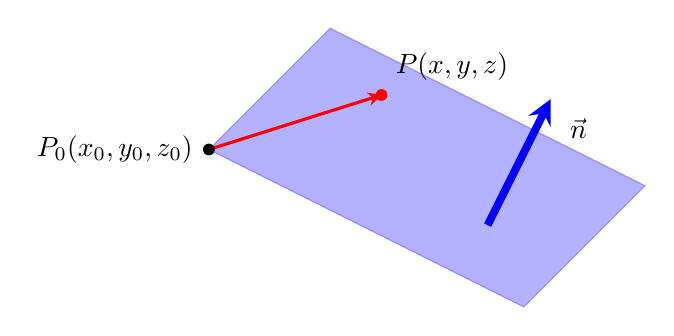
\begin{tikzpicture}[scale=1]

\filldraw[blue, opacity=0.3] (2,-0.5,2)--(2,-0.5,-2)--(-2,1.5,-2)--(-2,1.5,2)--cycle;

    \draw[->,line width=1mm, -stealth, blue](0,-1,-2)--(0.8,0.6,-2) ;%normal to grey
    
    \node[fill,red,circle,inner sep=1.5pt,label={above right:$P(x, y, z)$}] at (0,2,1.5) {};
    \node[label={below right:$\vec{n}$}] at (0.8,0.6,-2) {};
    
    \draw[->,line width=0.4mm, -stealth, red](-2,1.5,2)--(0,2,1.5) ;
    
    \node[fill,circle,inner sep=1.5pt,label={left:$P_0(x_0, y_0, z_0)$}] at (-2,1.5,2) {};
     \end{tikzpicture}
          
     \end{image}
 
Let $\vec{n}=\begin{bmatrix}a\\b\\c\end{bmatrix}$.  By ``head-tail" formula (Formula \ref{form:headminustailr3} of VEC-M-0010), we have: $\overrightarrow{P_{0}P} = \begin{bmatrix}
x - x_{0}\\
y - y_{0}\\
z - z_{0}
\end{bmatrix}$. So, $P(x, y, z)$ lies in the plane if and only if
$$\begin{bmatrix}a\\b\\c\end{bmatrix}\dotp\begin{bmatrix}
x - x_{0}\\
y - y_{0}\\
z - z_{0}
\end{bmatrix}=a(x-x_0)+b(y-y_0)+c(z-z_0)=0$$
We summarize this result as a theorem.

\begin{theorem}\label{th:scalareqofplane}
The plane through $P_{0}(x_{0}, y_{0}, z_{0})$ with a normal vector $\vec{n} = 
\begin{bmatrix}
a\\
b\\
c
\end{bmatrix}
\neq \vec{0}$ 
 is given by
\begin{equation}\label{eq:plane}
a(x - x_{0}) + b(y - y_{0}) + c(z - z_{0}) = 0
\end{equation}
\end{theorem}

\begin{example}\label{ex:planewithnormalvector}
Find an equation of the plane through $P_{0}(1, -1, 3)$ with $\vec{n} = 
\begin{bmatrix}
3\\
-1\\
2
\end{bmatrix}$
 as a normal vector.
\begin{explanation}
  Here the equation becomes
\begin{equation*}
3(x - 1) - (y + 1) + 2(z - 3) = 0
\end{equation*}
This simplifies to $3x - y + 2z = 10$.
\end{explanation}
\end{example}

As demonstrated in Example \ref{ex:planewithnormalvector}, we can distribute coefficients $a$, $b$ and $c$  of equation (\ref{eq:plane}) as follows:
$$ax-ax_0+by-by_0+cz-cz_0=0$$
Setting $d = ax_{0} + by_{0} + cz_{0}$, shows that every plane with a normal vector $\vec{n} =
\begin{bmatrix}
a\\
b\\
c
\end{bmatrix}$
 has a linear equation of the form
\begin{equation} \label{eq:eqofline} 
ax + by + cz = d
\end{equation}
for some constant $d$. Conversely, the graph of this equation is a plane with $\vec{n} =
\begin{bmatrix}
a\\
b\\
c
\end{bmatrix}$ as a normal vector (assuming that $a$, $b$, and $c$ are not all zero).


\begin{example}\label{ex:planeparalleltoplane}
Find an equation of the plane through $P_{0}(3, -1, 2)$ that is parallel to the plane with equation $2x - 3y = 6$.


\begin{explanation}
The plane with equation $2x -3y = 6$ has normal $\vec{n} =
\begin{bmatrix}
2\\
-3\\
0
\end{bmatrix}$. Because the two planes are parallel, $\vec{n}$ serves as a normal for the plane we seek, so the equation is $2x - 3y = d$ for some $d$ by (\ref{eq:eqofline}). Insisting that $P_{0}(3, -1, 2)$ lies on the plane determines $d$; that is, $d = 2 \cdot 3 - 3(-1) = 9$. Hence, the equation is $2x - 3y = 9$.
\end{explanation}
\end{example}

\section{Practice Problems}

\begin{problem}
Find an equation for each plane described below.

  \begin{problem}
  The plane has a normal vector $\vec{n}=\begin{bmatrix}2\\-3\\1\end{bmatrix}$ and the plane passes through the point $(4, 4, -3)$.
  
  Answer: $$\answer{2}x+\answer{-3}y+\answer{1}z=\answer{-7}$$
  \end{problem}
  
  \begin{problem}
  The plane contains the point $(-1, 3, 0)$ and is parallel to the plane described by $2x-5y+4z=7$.
  
  Answer:
  $$\answer{2}x+\answer{-5}y+\answer{4}z=\answer{-17}$$
  \end{problem}
  
  \begin{problem}
  The plane contains the point $(2, 0, 5)$ and is parallel to the $xz$-plane.
  
  Answer:
  $$\answer{0}x+\answer{1}y+\answer{0}z=\answer{0}$$
  \end{problem}

\end{problem}

\begin{problem}
How many planes satisfying each set of conditions are there?

\begin{problem}
Planes containing $(1, 2, 3)$ and $(4, 5, 6)$ with a normal vector $\vec{n}=\begin{bmatrix}-9\\-9\\-9\end{bmatrix}$.
\begin{multipleChoice}
 \choice[correct]{0}
 \choice{1}
 \choice{Infinitely Many}
 \end{multipleChoice}
\end{problem}

\begin{problem}
Planes containing $(0,2, 4)$, $(-1, 5, 3)$, $(4, 9, 1)$.
\begin{multipleChoice}
 \choice{0}
 \choice[correct]{1}
 \choice{Infinitely Many}
 \end{multipleChoice}
\end{problem}

\begin{problem}
Planes containing $(-1, 3, 5)$, $(1, 3, 6)$, $(3, 3, 7)$.
\begin{multipleChoice}
 \choice{0}
 \choice{1}
 \choice[correct]{Infinitely Many}
 \end{multipleChoice}
\end{problem}

\end{problem}

\end{document} 